\documentclass[mémoire.tex]{subfiles}
\begin{document}
\section{Méthodes topologiques}

\todo{paragraphe introductif}

\subsection{Introduction à la théorie du degré}

Plaçons nous, dans un premier temps, en dimension finie et considérons un ouvert $U$ de $\R^n$, $f\in C^0(\bar{U},\R^n)$ et $y\notin f(\partial U)$ et supposons qu'on veuille construire une fonction $\operatorname{deg}$ qui "compte" le nombre de de solutions de l'équation $f(x)=y$ dans $U$. Faisons une petite analyse de la situation: remarquons d'abord qu'on doit avoir la \coldef{normalité}
\begin{equation*}
    \forall y\in U,\operatorname{deg}(\operatorname{Id},U,y)=1
\end{equation*}

En effet, dans ce cas la seule solution est $x=y$. Mainenant, si on a deux sous ensembles ouverts de $U$, $V_1$ et $V_2$ et qu'ils sont disjoints. Supposons de plus que toutes les solutions soient dans $V_1$ ou $V_2$ et qu'elles sont en nombre fini, alors on aimerait bien avoir \coldef{l'additivité}

\begin{equation*}
    \operatorname{deg}(f,U,y)=\operatorname{deg}(f,V_1,y)+\operatorname{deg}(f,V_2,y)
\end{equation*}

Le lecteur familier avec la topologie trouvera particulièrement naturel d'exiger une notion \coldef{d'invariance par homotopie}. Précisons: on dira que $f$ et $g\in C^0(\bar{U},\R^n)$ sont homotopes si on peut trouver

\begin{equation*}
    H\in C^0([0,1]\times\bar{U},\R^n): H(0,\cdot)=f \text{ et } H(1,\cdot)=g
\end{equation*}
Informellement, on déforme continûment $f$ vers $g$. Attention, on ne peut pas déformer comme on veut, il faut que cette déformation n'affecte pas l'ensemble des solutions. On formule alors une troisième condition, ainsi, si on a 
\begin{equation*}
    H\in C^0([0,1]\times \bar{U},\R^n), y\in C^0([0,1],\R^n): \forall t\in [0,1], y(t)\notin H(t,\partial U)
\end{equation*}
alors  on voudrait que 

\begin{equation*}
    \operatorname{deg}(H(t,\cdot),U,y(t))
\end{equation*}
Soit toujours le même. Notez qu'en plus la fonction, on s'autorise aussi à bouger la "cible", mais on s'interdit de toucher la frontière !
de façon remarquable, en dimension finie, il n'y a qu'une seule fonction qui possède ces propriétés ! On peut donc parler "du" degré. On l'appelle le \coldef{degré de Brouwer}

\begin{definition}
    Si $U\subseteq \R^n$ est ouvert et borné, si $f\in C^0(\bar{U})\cap C^1(U)$ et $y\in \R^n\setminus f(\partial U \cup S_f(U))$ alors on pose 
    \begin{equation*}
        \operatorname{deg}_B(f,U,y)=\sum_{x\in f^{-1}(y)} \operatorname*{sign} \det df(x)
    \end{equation*}
\end{definition}
On peut montrer que cette fonction remplit bien les 3 
conditions et que c'est la seule. Ensuite, via le 
\colprop{théorème de Morse-Sard} et quelques techniques 
d'approximation classiques, on peut généraliser cette 
fonction à $C^0(\bar{U})$, voir \cite{KlausNonLin85} pour 
les détails. Notez que les 3 conditions mènent à une 
fonction qui ne compte pas vraiment le nombre de 
solutions, mais associe un signe à chacune d'entre elles. 


\subsection{Approche historique: le degré de Leray-Schauder}
Il est impossible de généraliser la notion du degré de Brouwer aux espaces de Banach. Pour le voir, nous montrons un cas particulier du théorème du point fixe en utilisant uniquement les propriétés du degré et montrons ensuite qu'il ne s'applique pas en dimension infinie
\begin{proposition}
    si $r>0$ et $f\in C^0(\bar{B(0,r)},\bar{B(0,r)})$ alors $f$ admet un point fixe
\end{proposition}
\begin{preuve}
    S'il existe $x\in\partial \bar{B(0,r)}$ tel que $f(x)=x$, on a terminé. Sinon,
    Considérons 
    \begin{equation*}
        H: [0,1]\times \bar{B(0,r)}\rightarrow \R^n: (t,x)
        \mapsto x-tf(x)\text{ et } y(t)=0
    \end{equation*}
    C'est une homotopie entre $\operatorname{Id}-f$ et 
    l'identité et $0\notin H([0,1]\times\partial \bar{B(0,r)})
    $ car, si $x\in\partial \bar{B(0,r)}$, $H(t,x)=x-f(x)\neq 
    0$ par hypothèse et si $0\leq t<1$
    \begin{equation*}
        |H(t,x)|\geq |x|-t|f(x)|\geq (1-t)r>0
    \end{equation*}
    et donc
    \begin{equation*}
        \operatorname*{deg}(\operatorname{Id}-f,B(0,r),0)
        =\operatorname*{deg}(\operatorname{Id},B(0,r),0)=1
    \end{equation*}
    et donc il existe $x\in B(0,r)$ tel que $x-f(x)=0$
\end{preuve}

Un petit contre exemple en dimension infinie
\begin{exemple}
    Considérons $X=l_\infty$ 
    \begin{equation*}
        f: B(0,1)_{\infty}\rightarrow B(0,1)_{\infty}
    , (x_i)_{i\in\mathbb{N}}\mapsto 
        (1-||x||_{\infty},\sqrt{|x_1|},\sqrt{|x_2|},\cdots)
    \end{equation*}
    On vérifie facilement que $f$ est continue. Supposons donc qu'elle a un point fixe $y$, on aurait alors 
    \begin{equation*}
        y_1= 1- ||y||_{\infty}\text{ et, si $k\geq 2$  } y_k = |y_1|^{\frac{1}{2^{k-1}}}
    \end{equation*}
    Si $||y||_\infty=1$,  alors tous les $y_k$ sont nuls, absurdité. Si $||y||_\infty<1$, alors $y_1$ et la suite converge vers 1, absurdité car cela impliquerait $||y||_{\infty}=1$
\end{exemple}
\begin{corollaire}
    Il n'existe pas d'équivalent au degré de Brouwer en dimension infinie.
\end{corollaire}
Il faut alors restreindre l'ensemble des fonctions sur lequel on va travailler si on veut espérer définir une notion de degré. C'est le travail effectué par  Juliusz Schauder et  Jean Leray pendant les années 30, nous consacrons les prochaines paragraphes à en faire la synthèse.
Le degré de Leray-Schauder est défini sur les \coldef{ perturbations compactes de l'identité} i.e on suppose $F$ de la forme $I-G$ avec $G$ une application compacte , il a alors obtenu le résultat suivant
(qu'on énonce sans preuve) 

\begin{theobox}{Leray-Schauder}{}
    Soit $X$ un espace de Banach et 
    \begin{equation*}
        A=\left\{
            (I-G,U,y): U \subseteq\mathcal{B}(X)\text{ et ouvert },G\in\mathbb{K}(\bar{U}),y\notin (I-G)(\partial U)
        \right \}
    \end{equation*}
    l'ensemble des \coldef{triplets admissibles}
    il existe une unique fonction 
    \begin{equation*}
        \operatorname{deg}: A\rightarrow \mathbb{Z}
    \end{equation*}
    satisfaisant la normalité, l'invariance par homotopie et l'additivité.
\end{theobox}


Avec ce degré, on peut obtenir des résultats globaux de Bifurcation sa construction nécéssite pas mal de lemmes techniques, les démonstrations sont laborieuse et les résultats sont plus faibles que ceux obtenus avec la notion de degré plus récente présentée ci-dessous

\subsection{Le degré de Furi}
\subsubsection{Orientation de fonction de Fredholm d'indice nul}
Nous allons introduire une notion d'orientation pour les fonctions de Fredholm. Cette dernière, proposée par Furi dans \cite{BenevieriFuri1998}, a ensuite été mobilisée dans \cite{BenevieriFuri2001} pour obtenir des résultats de bifurcation. Nous présentons ainsi les idées de ces 2 papiers.
\begin{definition}
    Si $X,Y$ sont des espaces de Banach et  $D\in\mathcal{F}_0(X,Y)$ alors $E\in L(X,Y)$ est un \coldef{correcteur } de $D$ si $D+E$ est un isomorphisme d'espace vectoriel et si son image est de dimension finie. On pose $\mathcal{C}(D)$ l'ensemble des correcteurs de $D$
\end{definition}
On remarque que $\mathcal{C}(D)$ n'est jamais vide, en effet, si on écrit $X=\ker D\oplus X_0$ et $Y=\operatorname*{im} D \oplus Y_0$, on sait que $\ker D$ et $Y_0$ sont isomorphes, notons $A_0$ l'isomorphisme, on remarque alors que 
\begin{equation}\label{correcteur-exemple}
    A:  X\rightarrow Y, x_1+x_2\mapsto A_0(x_1)
\end{equation}
répond à la question. En effet, il est injectif car $Y_0\oplus \operatorname*{im} D=Y$ et il est surjectif car une perturbation de rang fini d'un opérateur de Fredholm ne change pas l'indice.
Dans la suite de cette section on suppose $D$ comme dans la définition précédente.
Avant de pouvoir définir l'orientation, il nous faut une notion de "avoir la même orientation", on fait ça en définissant une relation d'équivalence sur $\mathcal{C}(D)$

\begin{lemme}
    Soient $D\in\mathcal{F}_0(X,Y)$ et $E,E'\in \mathcal{C}(D)$. Si on pose $\phi_{E,E'}=(D+E')^{-1}(D+E)$
    l'opérateur
    \begin{equation*}
        F= \operatorname{Id}_X -\phi_{E,E'}
    \end{equation*}
    a une image de dimension finie
\end{lemme}

\begin{preuve}
   Notons d'abord que 
   \begin{equation*}
        (D+E')F= (D+E')-(D+E)=E'-E
   \end{equation*}
   donc $\im F=\im (E-E')$. Et du fait que 
   \begin{equation*}
        \dim \im (E-E')\leq \dim (E+E')\leq \dim(E)+\dim(E'),
   \end{equation*}
   on conclut.
\end{preuve}




\begin{lemme}
    Soit $F$ comme dans le lemme précédent, alors pour tous $X_0,X_1\subseteq  X$ sous-vectoriels de dimension 
    finie contenant $\im F$
    \begin{equation*}
        \det \phi_{E,E'}|_{X_0}= \det \phi_{E,E'}|_{X_1}
    \end{equation*}
    avec la convention que si $X_0=\{0\}$,  $\det \phi_{E,E'}|_{X_0}=1$
\end{lemme}
\begin{preuve}
    Notez que $\phi_{E,E'} =I-F$ est un isomorphisme, que $(I-F)(X_0)\subseteq X_0$, donc $(I-F)|_{X_0}: X_0\rightarrow X_0$ est un automorphisme d'un espace vectoriel de dimension finie, la notion de déterminant à donc un sens. Supposons d'abord avoir $X_0\subseteq X_1$, on le complémente par $X'_0$, i.e 
    \begin{equation*}
        X_1=X_0\oplus X'_0
    \end{equation*}
    On décompose alors $(I-F)_{X_1}$ comme ceci
    \begin{equation*}
            \begin{pmatrix}
        \operatorname{Id}_{X'_0} & 0 \\
        -\pi_F & (I-F)_{E_0} 
        \end{pmatrix}
    \end{equation*}
où  $\pi_F$ est la projection sur $X_0$ de  $F_{X'_0}$, on conclut immédiatement. Maintenant, dans le cas général, notez que $X_0\cap X_1$ contient $\im F$ et est de dimension finie. On applique alors le résultat obtenu deux fois 
\begin{equation*}
    \det (I-F)|_{X_0}= \det (I-F)|_{X_1\cap X_0}=\det (I-F)|_{X_1}
\end{equation*}
\end{preuve}

Dans la suite, on s'autorisera parfois à écrire $\det \phi_{E,E'}$, en laissait implicite le sous espace $X_0$.



\begin{definition}
    dans les conditions des deux lemmes précédents, 
    on dit que les correcteurs  $E$ et  $E'$  sont 
    $D$-\coldef{équivalents} si $\det (\phi_{E,E'})>0$, on écrira  $E\sim_{D} E'$
\end{definition}
\begin{proposition}
    $\sim_D$ est une relation d'équivalence sur $\mathcal{C}(D)$
\end{proposition}
\begin{preuve}
    La réfléxivité et la transitivité sont évidentes,on montre alors la transitivité. Soient donc $E,F,G\in\mathcal{C}(D)$ tels que $E\sim_D F$ et $F\sim_D G$ on considère alors un sous vectoriel de dimension fini $X_0$ content les images de $I-\phi_{E,F},I-\phi_{F,G},I-\phi_{E,G}$ , il suifft alors de remarquer que 
    \begin{equation*}
        \det \phi_{E,G}|_{X_0}=
        \det \phi_{F,G}\phi_{E,F}|_
        {X_0}=
        \det \phi_{F,G}|_{X_0}
        \cdot \det \phi_{E,F}>0
    \end{equation*}
    donc $E\sim_{D} G$ 
\end{preuve}

Il  de plus clair que cette relation d'équivalence partitionne 
$\mathcal{C}(D)$ en deux classes d'équivalence. Notez que si $D_1$ et $D_2$ peuvent être composés et que si $E_1$ et $E_2$ sont des correcteurs de $D_1$ et $D_2$ respectivement, alors $D_2E_1+ E_2E_1+ E_2D_1$ est un correcteur de $D_2D_1$, de fait 

\begin{equation*}
    D_2D_1+ D_2E_1+ E_2E_1+ E_2D_1 =(D_1+E_1)(D_2 + E_2)
\end{equation*}


\begin{definition}
    Une \coldef{orientation} de $D\in\mathcal{F}_0(X,Y)$ est une des 2 classes d'équivalence de $\mathcal{C}(D)$. Un \coldef{opérateur orienté} est une paire $(D,c)$ où $c$ est une oreitnation. Si $(D,c)$ est orienté, un correcteur sera dit \coldef{positif} s'il est dans $c$ et négatif sinon. On pose alors $\mathcal{C}_{+}(D)$ l'ensemble des correcteurs positifs et $\mathcal{C}_{-}(D)$ les négatifs. Lorsque $D$ est un isomorphisme, $0$ est un correcteur, on définit alors \coldef{l'orientation naturelle} $\nu(D)$ de $D$ comme étant la classe d'équivalence contenant $0$. Si $(D,c)$ est isomorphisme orienté, on pose $\operatorname{sgn}D=1$ si $0\in c $, et $-1$ sinon , si $D$ n'est pas un isomorphisme, on pose alors $\operatorname{sgn}D=0$
\end{definition}
\begin{definition}
    Si $(D_1,c_1)$ et $(D_2,c_2)$ sont des opérateurs orientés, on note $c_2\circ c_1$ l'orientation de $D_2\circ D_1$ telle que
    \begin{equation*}
        D_2E_1+ E_2E_1+ E_2D_1\in  c_2\circ c_1
    \end{equation*}
    où $E_1\in c_1$ et $E_2\in c_2$. On vérifie 
    facilement que ça ne dépend pas du choix des 
    $E_1$, $E_2$ La composition de deux opérateurs 
    orientés sera, sauf si mention du contraire, 
    la précédente. 
\end{definition}

Il est enrichissant de remarquer 
que la catégorie $\mathcal{G}(D)$ 
ayant pour objets les éléments de 
$\mathcal{C}(D)$ et comme 
morphismes les $(\phi_{E,F})_{E,F\in\mathcal{C}(D)}$ est un groupoïde. Si on considère la catégorie correspondant à $\mathbb{Z}_2$, i.e la catégorie n'ayant qu'un seul objet $o$ , $+1,-1$ comme morphismes et la multiplication comme loi de composition , qu'on note $\mathbf{B}\mathbb{Z}_2$
\footnote{C'est le "delooping" du groupe $\mathbb{Z}_2$, le lecteur intéressé peut consulter l'article nLab \url{ https://ncatlab.org/nlab/show/delooping} }
alors 

\begin{equation*}
    \operatorname*{Sign}: \mathcal{G}(D)\rightarrow \mathbf{B}\mathbb{Z}_2, E\mapsto o, \phi_{E,E'}\mapsto \operatorname*{sgn}\det \phi_{E,E'}
\end{equation*}

est un foncteur donc $\mathcal{G}^+(D)$, la catégorie $\mathcal{G}(D)$ ou on retire les les morphismes dont le determinant restreint est négatif, est un sous groupoïde (c'est même un sous groupoïde normal) de $\mathcal{G}(D)$. Il est clair que ce groupoïde à axactement deux composantes connexes, qui correspondent donc aux choix possibles d'orientation\\
Soit $(D,c)$ un opérateur orienté, via Hanh-Banach, on peut supposer que le correcteur $A$ donné en \ref{correcteur-exemple} est continu, on peut de plus supposer qu'il est positif. Maintenant, $D+A$ est un isomorphisme d'espaces de Banach et il existe un voisinage (pour la topologie des opérateurs) $V_D$ tel que si $D'\in V_D$, alors $A$ est un correcteur de $D'$, on appelle alors \textcolor{color-def}{l'orientation induite par $(D,c)$} sur $D'$ celle qui fait de $A$ un correcteur positif \\
On définit maintenant l'orientation pour une famille continue d'opérateurs de Fredholm
\begin{definition}
    Soit $(\Lambda,\mathcal{T})$ un espace topologique et $h\in C^0(\Lambda,\mathcal{F}_0(X,Y))$,
    $\alpha_{\lambda}$
    est une 
     \textcolor{color-def}{orientation} 
    si  pour tout $\lambda\in\Lambda$, $\alpha_{\lambda}\in\mathcal{C}(h(\lambda))/\sim_{h(\lambda)}$ et il existe $A_{\lambda}\in\alpha_\lambda$ qui est correcteur positif (pour l'orientation induite) de $h(\lambda')$ si $\lambda'$ est dans un voisinnage de $\lambda$. Une famille est alors dite \textcolor{color-def}{orientable} si il existe une orientation. Un sous ensemble $\mathcal{D}$ d'opérateurs de Fredholm d'indice 0 est orientable si l'inclusion $\iota : \mathcal{D}\rightarrow \mathcal{F}_0(X,Y)$ est orientable
\end{definition}

\begin{lemme}
    Dans les condition de la définition précédente, si $\Lambda$ est connexe, et si $h$ est orientable, alors $h$ admet exactement deux orietations 
\end{lemme}

\begin{preuve}
    Soit $\alpha_\lambda$ une orientation de $h$, et supposons que $\alpha'_\lambda$ coïncident avec $\alpha$ sur une partie $\Omega$ de $\Lambda$ et montrons qu' $\Omega$ est ouvert. Soit alors $\lambda_0\in\Omega$, par définition, il existe des voisinages de $\lambda_0$ $V_1$,$V_2$ et $A_1\in\alpha'(\lambda_0)$, 
    $A_2\in\alpha'(\lambda_1)$ qui sont des correcteurs positifs pour $h(\lambda')$ si $\lambda'$ est dans $V_1$ ou $V_2$, respectivement. Il suffit alors de remarquer que $\alpha$ et $\alpha'$ coïncident sur $V_1\cap V_2$. De façon identique, l'ensemble sur lesquels les orientations sont opposées est un ouvert, on conclut immédiatement
\end{preuve}

\begin{remarque}
    Notez que cette notion d'orientabilité est une généralisation de la notion d'orientabilité d'une variété plongée $M$ de dimension finie $n$: en effet, il suffit de considérer
    \begin{equation*}
        h: M\rightarrow L(\R^n,\R^n), x\mapsto \pi^{N_x} 
    \end{equation*}
    avec  $\pi^{N_x}$ la projection sur l'espace normal $N_xM$
\end{remarque}

\begin{definition}
    Soit $U\subseteq X$ un ouvert et $F: U\rightarrow X$ une fonction de Fredholm d'indice zéro. Une \textcolor{color-def}{orientation} de $F$ est simplement une orientation de $DF$ , et $F$ est \textcolor{color-def}{orientable} si $DF$ l'est. Si $F$ est un difféomorphisme, alors $F$ possède une orientation naturelle, notée $\nu$
\end{definition}

\subsubsection{Construction du degré de Furi}

On peut maintenant construire le degré de Furi
\begin{definition}
    Soit $F:X\rightarrow Y$ une fonction orientable et $y\in Y$, le triplet $(F,X,y)$ est 
    \textcolor{color-def}{admissible} si $F^{-1}(y)$ est compact. Si $U$ est un ouvert de $X$, on dit que le triplet $(F,U,y)$ est
    \textcolor{color-def}{admissible} si $F^{-1}(y)\cap U$ est compact et \textcolor{color-def}{fortement admissible } si $F$ admet une extension $F'$ continue $\bar{U}$, propre, et telle que $y\notin F(\partial U)$
\end{definition}

Dans la suite, on suppose $F$ orientée.Du fait que les fonctions de Fredholm sont localement propre \ref{propre-fred}, l'admissiblité du triplet $(F,X,y)$ implique l'existance d'un voisinnage ouvert de $F^{-1}(y)$ qui rend le triplet $(F,U,y)$ fortement admissible 

\begin{definition}
    Soit $U\subseteq X$ un ouvert et  $H\in C^0(U\times [0,1],Y)$ continûment dérivable par rapport à la première variable. $(H,\alpha)$ est une \coldef{homotopie orientée} si $\alpha$ est une orientation de $D_1 H$
\end{definition}

On adapte alors les propriétés qu'on voudrait avoir pour  le degré \\
Les conditions d'\coldef{additivité} et de \coldef
{normalité} restent les mêmes que pour le degré de Brouver \coldef{L'invariance par 
homotopie} devient une \coldef{invariance par homotopie 
orientée}:\\  Soit $H: X\times [0,1]\rightarrow Y$ une homotopie orientée et $y\in C^0([0,1],Y)$, si l'ensemble 
\begin{equation*}
    \left\{(x,t)\in X\times [0,1]: H(x,t)=y(t) \right\}
\end{equation*}
est compact alors $\deg (H_t,X,y(t))$ est bien défini pour et ne dépend pas de $t\in [0,1]$\\
La propriété suivante est évidente pour le degré de Brouwer, mais à expliciter  en dimension infinie, il s'agit de \coldef{l'invariance topologique}: Si $(F,X,y)$ est admissible et $\varphi: W\rightarrow X$, $\psi: Y\rightarrow Z$ sont des difféomorphismes naturellement orientés alors 
\begin{equation*}
    \deg(F,X,y)=\deg(\psi F \varphi, W, \psi(y))
\end{equation*}

Enfin, une propriété qui nous permet de faire l'analogue de l'analogue de la réduction de Lyapunov-Schmidt
\begin{definition}
   Si $Y_0$ est un sous espace de $Y$,  $F:X\rightarrow Y$ est \coldef{transverse à $Y_0$ en $x$ }
   \begin{equation*}
    Y_0+\im DF(x)=Y.
   \end{equation*}
   On dit qu'elle est \coldef{transverse à $Y_0$} si elle est transverse en tout point de $F^{-1}(Y_0)$
   on notera dans ce cas $F\pitchfork Y_0$
\end{definition}
\begin{remarque}\label{rem-trans}
    Si $G:X\rightarrow Y$ est de 
    Fredholm en $x_0$ alors il 
    existe un sous espace de 
    dimension finie $Y_0$ tel que 
    $G$ est transverse à $Y_0$. 
    L'ensemble des applications 
    surjectives continues entre 
    deux espaces de Banach étant 
    un ouvert (conséquence directe 
    du théorème de l'application 
    ouverte), $G$ est transversale 
    à $Y_0$ sur un ouvert 
    contenant $x_0$. En fait, 
    $D\in\mathcal{L}(X,Y)$ est de 
    Fredholm si et seulement si il 
    existe $X_0^{*}\subseteq X^*$ 
    et $Y_0\subseteq Y$ de 
    dimensions finis tels que 
    $D\pitchfork Y_0$ et $D^{*}
    \pitchfork X_0^{*}$ 
\end{remarque}
\coldef{Réduction}: si $F:X\rightarrow Y$ est orientée et $F\pitchfork Y_0$, alors on pose  $F_1$ la restriction de $F$ à $X_0=F^{-1}(Y_0)$, alors on veut que
\begin{equation*}
    \deg (f,X,y)=\deg(f_1,X_0,y)
\end{equation*}
On aussi la propriété \coldef{d'excision} qui découle directement de l'additivité:
 si $(F,X,y)$ est admissible et $U$ est un voisinage ouvert de $F^{-1}(y)$ alors 
\begin{equation*}
    \deg(F,X,y)=\deg(F,U,y)
\end{equation*}

\begin{definition}
    Si $(F,X,y)$ est $y$ est une valeure régulière de $F$. alors on pose
    \begin{equation*}
        \deg_f(F,X,y)=\sum_{x\in f^{-1}(y)} \operatorname{sgn}DF(x)
    \end{equation*}
    la quantité ci-dessus est bien définie car $F^{-1}(y)$ est un ensemble discret et fini
\end{definition}


On vérifie facilement que la 
fonction ci-dessus respecte les 
conditions attendues.\\


\begin{lemme}
    Soit $(F,X,y)$ un triplet 
    admissible et $V$ un ouvert de 
    $Y$ contenant $y$, il  existent 
    $Y_0\subseteq Y$ de dimension 
    finie et $U\subseteq F^{-1}(V)
    $ un ouvert contenant 
    $F^{-1}(y)$ tel que $F$ est 
    transverse à $Y_0$ sur $U$. En particulier, $X_0=F^{-1}(Y_0)\cap U$ est une variété différentielle de la même dimension que $Y_0$
\end{lemme}
\begin{preuve}
    Soit $x\in F^{-1}(y)$, 
    considérons $Y_x$ un sous 
    espace de dimension fini de 
    $Y$ tel que $F$ est transerse 
    $Y_x$ en $x$. Au vu de la remarque \ref{rem-trans}, il existe alors un ouvert $U_x$ sur 
    lequel $F$  est transverse à 
    $Y_x$. Du fait que $F^{-1}(y)$ est compact, on peut trouver $U_1,\cdots, U_k$ des ouverts inclus dans $F^{-1}(V)$ et des sous espaces $Y_1,\cdots , Y_k$ de dimensions finies tel que $F$ est transverse à $Y_i$ sur $U_i$ pour $1\leq i\leq k$ et $Y_0=\sum_{i=1}^{k} Y_k$
    convient.\todo{Prouver dimension}
\end{preuve}


\begin{definition}
    Soient $X_0,Y_0$ comme le lemme ci-dessus et $F_0:X_0\rightarrow Y_0$ la restriction de $F$ à $X_0$. $Y_0$ est orientable, $F$ est orientable donc $X_0$ est orientable, ainsi, $F_0$ induit une orientation sur $X_0$ et $Y_0$, on dirait que $X_0$ et $Y_0$ sont orientés \coldef{selon $F$}
\end{definition}

\begin{lemme}
    Soit $(F,M,y)$ un triplet admissible avec $y$ une valeure régulière, $Y_0$ un sous espace de dimension finie tel que $f\pitchfork Y_0$ alors $X_0=F^{-1}(Y_0)$ est une variété de même dimension que $Y_0$ orientable. De plus, si on oriente $X_0$ et $Y_0$ selon $F$, alors 
    \begin{equation*}
        \deg_f(F,X,y)=\deg_B(F,X,y)
    \end{equation*}
\end{lemme}

\begin{preuve}
    \todo{écrire la preuve}
\end{preuve}

\begin{lemme}
    Si $(F,M,y)$ est fortement 
    admissible, et si $U_1,U_2$ 
    sont des voisinages de $F^{-1}
    $, alors il existe un 
    voisinage $V$ de $y$ tel que 
    pour toute paire de valeur 
    régulière $y_1,y_2$, on aie 
    \begin{equation*}
        \deg_f(F,U_1,y_1)= \deg_f(F,U_1,y_2)
    \end{equation*}
\end{lemme}
\begin{preuve}
    \todo{Preuve}
\end{preuve}

\begin{theobox}{}{}
    La fonction $\deg_f$ respecte les conditions de normalité, d'additivité, d'invariance topologique , d'invariance par homotopie orientée et de réduction
\end{theobox}
\begin{preuve}
    \todo{Preuve}
\end{preuve}

\begin{definition}
    Soit $U$ un ouvert de $X\times \R$, 
    $F:U\rightarrow Y$ est une \coldef{famille 
    continue de fonctions de Fredholm d'indice zéro} 
    si pour tout $\lambda$ tel que $U_{\lambda}
    =\left\{ x\in X: (x,\lambda)\in U\right\}$ est 
    non vide, $F(\cdot,\lambda): U_{\lambda}
    \rightarrow Y$ est de Fredholm d'index nul et si 
    $D_2F$ est coninue sur $U$
\end{definition}
\begin{remarque}
    Notez que cette condition est plus faible que celles des chapitres précédents étant donné qu'on ne demande pas à $F$ elle même d'être régulière sur une partie du produit $X\times \Lambda$
\end{remarque}

 \todo{Justifier le sens du determinant dans le thm suivant}


\begin{theobox}{}{}
    Soit $F:U\rightarrow Y$ une famille d'index zéro et ayant une branche triviale de solutions et soit $A\in\mathcal{C}(D_2F(0,\lambda_0)) $ si la fonction 
    \begin{equation*}
        f: \R\rightarrow\R, \lambda\mapsto \det ((DF(0,\lambda)+A)^{-1}D_2F(0,\lambda))
    \end{equation*}
    change de signe en $\lambda_0$, alors c'est un point de bifurcation. 
\end{theobox}
\begin{preuve}
    Supposons que $\lambda_0$ n'est pas un point de 
    bifurcation, alors il existe un voisinage ouvert de $(0,
    \lambda_0)$ ne contenant que des solutions 
    triviales, qu'on peut supposer de la forme 
    \begin{equation*}
        U=]\lambda_0-\delta,\lambda_0+\delta[\times B_{r}(0)\text{ avec $\delta>0$ et $r>0$}
    \end{equation*}
    et on a donc 
    \begin{equation*}
        U\cap F^{-1}(0)=]\lambda_0-\delta,\lambda_0+\delta[\times \left\{0\right\}
    \end{equation*}
    Soit alors $A\in\mathcal{C}(D_2F(0,\lambda_0))$, étant donné que l'ensemble des isomorphismes est ouvert, on peut supposer, quitte à réduire $\delta$, que $A\in\mathcal{C}(DF(x,\lambda))$ si $(x,\lambda)\in U$. Donc $A$ induit une orientation de $F$ sur $U$. étant donné que $B_r(0)\cap F^{-1}(0,\lambda)=\left\{0\right\}$ si $\lambda\in ]\lambda_0-\delta,\lambda_0+\delta[$, $\deg(F(\cdot,\lambda),B_r(0),0)$ et bien défini, et étant donné l'invariance par homotopie orientée, indépendant de $\lambda$.
    étant donné que la fonction $f$ change de signe en $\lambda_0$, $D_2F(0,\lambda)$ est un isomorphisme si $\lambda$ proche de $\lambda_0$.
    La définition du degré nous permet alors d'écrire
    \begin{equation*}
        \deg_f (F(\cdot,\lambda),B_r(0),0)=\operatorname*{Sign}D_2F(\cdot,\lambda)=\operatorname*{Sign} \det ((D_2F(0,\lambda)+A)^{-1}D_2F(0,\lambda))
    \end{equation*}
    si $\lambda\in ]\lambda_0-\delta,\lambda_0+\delta[ $.Le signe reste alors constant, contradiciton.
\end{preuve}
\subsubsection{Un résultat global via le degré de Furi}
Nous allons maintenant obtenir un résultat de Bifurcation global. Pour ce-faire, il nous faut d'abord montrer quelques lemmes techniques, à commencer par un résultat purement topologique, dû à [SOURCE]. Ce dernier dépend du résultat suivant, que nous admettons afin de ne pas alourdir l'exposé
\begin{proposition}\label{seperation-of-sets}
    Soit $(E,\mathcal{T})$ un espace compact séparé. Si $A$ et $B$ sont des sous ensembles fermés pour lesquels il n'existe pas de d'ouverts $U,V$ tels que $U\cap V=\emptyset$, $U\cup V=E$ et $A\subseteq U, B\subseteq V$, alors il existe un sous ensemble connexe $C$ tel que $A\cap C$ et $B\cap C$ sont non vides 
\end{proposition}
\begin{preuve}
    Voir [SOURCE]
\end{preuve}
\begin{lemme}
    Soit $(E,\mathcal{T})$ un espace topologique séparé localement compact  et $K\subseteq E$ compact et tel que $\partial K\neq \emptyset  $. Supposons de plus que pour tout sous ensemble compact  $K_1$ contenant $K$, $\partial K_1\neq \emptyset$. Alors $E\setminus K$ contient un ensemble connexe $C$ tel que $\bar{C}$ n'est pas compact et $\bar{C}\cap K\neq \emptyset$.
\end{lemme}
\begin{figure}[htbp]
    \centering
    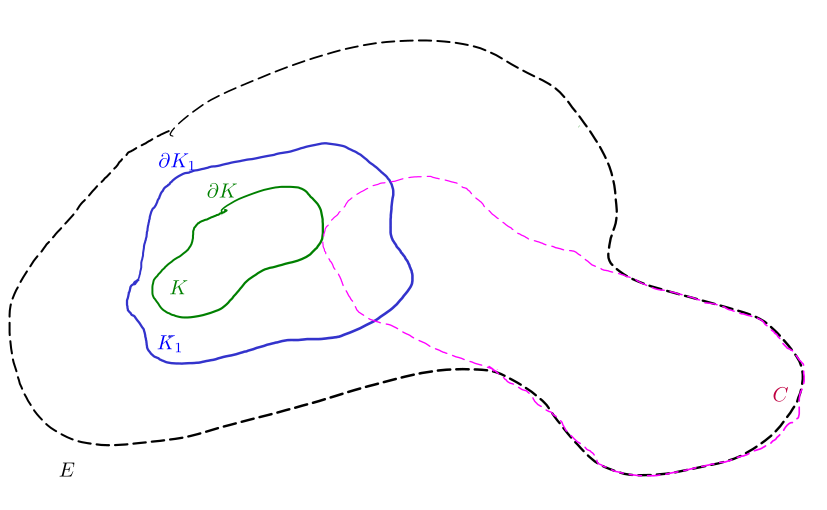
\includegraphics[width=0.6\textwidth]{figures/lemme-topo_1.png}
\end{figure}
\begin{preuve}
    On commence par ajouter un 
    point à $E$, qu'on appelle 
    "$\infty$". On met ensuite une 
    topologie  $\mathcal{T}'$ sur 
    $E'=E\cup \left\{\infty\right\}$ en considérant 
    que les voisinages ouvert de "$\infty$" sont les 
    complémentaires des ensemble compacts, en 
    gardant les mêmes voisinages ouverts pour tous 
    les autres points, ce qui en fait un espace compact et séparé (c'est simplement le compactifié). Il suffit alors de trouver un 
    sous ensemble connexe $C$ de $E'\setminus(K\cup 
    \left\{\infty \right\}) $ et tel que $\infty\in 
    \bar{C}$. Supposons qu'un tel ensemble n'existe pas, du fait que $(E',\mathcal{T}')$ est compact et séparé, et au vu \ref{seperation-of-sets}, on peut trouver deux ensembles compacts $C_{\infty}\ni \infty $ et $C_{K}\supseteq K$ tels que $C_{K}\cup C_{\infty}=E'$, $C_{K}\cap C_{\infty}=\infty $. Mais alors, $C_{K}$ est un compact ouvert, donc de frontière vide, qui contient $K$, impossible. Donc il existe bel et bien un tel $C$
\end{preuve}
\begin{remarque}
    La condition du lemme précédent est vraie dès qu'on a un espace séparé, connexe et non compact $E$. En effet supposons avoir un compact $K_1$ qui contient $K$. Si on suppose $\partial K_1=\emptyset$ alors $K_1$ est ouvert fermé, étant donné qu'il est non vide, on doit avoir $K_1=E$, contradiction car $E$ non compact
\end{remarque}

\begin{lemme}
    Soit $F:U\rightarrow Y$ une 
    famille de fonction de 
    Fredholm orientée d'indice 
    zéro et $y:[0,1]\rightarrow Y$ un chemin continu. Si 
    \begin{equation*}
        K=\left\{ (\lambda,x): \lambda\in [0,1], F(\lambda,x)=y(\lambda)\right\}
    \end{equation*}
    est compact alors 
    \begin{equation*}
        \deg_f(F(\cdot,\lambda),U_{\lambda},y(\lambda))
    \end{equation*}
    ne dépend pas de $\lambda$
\end{lemme}
\begin{preuve}
    Il s'agit d'une conséqence des 
    propriétés d'excision et d'invariance 
    par homotopie\\
    \todo{Ecrire la preuve en détail}
\end{preuve}

Le résultat suivant est en fait une version plus puissante de \ref{propre-fred}

\begin{lemme}
    Soit $U$ un ouvert de $\R^n\times X$, et $F\in C^0(U,Y)$. Si $F$ est continument dérivable par rapport à $\lambda$ et si $D_2F$ est de Fredholm sur $U$, alors $F$ est localement propre
\end{lemme}
\begin{preuve}
    Soit $(x_0,\lambda_0)\in U$, étant donné que $D=D_2F(x_0,\lambda_0)$ est de Fredholm, il existe des sous espaces $X_0,Y_0$ tels que $X=\ker D\oplus X_0 $ et $Y=Y_0\oplus \im D$. On pose alors $\pi_1,\pi_2$ les projections naturelles associées avec la décomposition de $Y$. Un élément de $X$ (resp. $Y$) s'écrit comme $x_1+x_2$ (resp. $y_1+y_2$) avec $x_1\in \ker D$ (resp $y_1\in Y_0$) et 
    $x_2\in X_0 $ (resp $y_2\in\im D$) on pose alors
    \begin{equation*}
        F_1: U\times Y_0\rightarrow Y_0, (x_1,x_2,\lambda,y_1)\mapsto \pi_1(F(x_1,x_2,\lambda))-y_1
    \end{equation*}
    Et
    \begin{equation*}
        F_2:U\times \im D\rightarrow \im D,
        (x_1,x_2,\lambda,y_2)\mapsto \pi_2(F(x_1,x_2,\lambda))-y_2.
    \end{equation*}
    On pose $x_{1,0}+x_{2,0}=x_0$ et 
    $y_{1,0}+y_{2,0}=f(x_0,\lambda_0)$.
    Notez que
    \begin{equation*}
        (D_3 F_2)(x_{1,0},x_{2,0},\lambda_0,y_{2,0})=\pi_2(D_2F(x_0,\lambda_0)):X_0\rightarrow  \im D
    \end{equation*}
    est un isomorphisme. On peut donc 
    appliquer le théorème des fonctions 
    implicites, qui nous fournit un 
    voisinage fermé $A\times B\times C\times 
    D$ de $(x_{1,0},x_{2,0},\lambda_0,y_{2,
    0})$ dans lequel $F_2^{-1}(0)$ est le 
    graphe d'une fonction  continue 
    $g:A\times B\times D\rightarrow C$. Soit 
    alors $(x_{1,n},x_{2,n},\lambda_n)_
    {n\in\mathbb{N}}$ une suite de $A\times 
    B\times C$ telle que $F(x_{1,n},x_{2,n},
    \lambda_n)=(y_1)$, on veut montrer que $(x_{1,
    n},x_{2,n},\lambda_n)_
    {n\in\mathbb{N}}$ admet une sous suite 
    convergente. On peut supposer que $\lambda_n$ et $x_{1,n}$ converge ($A$ et $D$ de dimension finie)
\end{preuve}
\begin{definition}
    Soit $\gamma: [0,1]\rightarrow \mathcal{F}_0(X,Y)$ un chemin continu présente un \coldef{saut de signe} en $\lambda_0$ si,  étant donné $A\in\mathcal{C}(\gamma(\lambda_0))$ la fonction réelle
    \begin{equation*}
        \lambda\mapsto \det ((\gamma(\lambda)+A)^{-1}\gamma(\lambda))
    \end{equation*}
    change de signe en $\lambda_0$
\end{definition}
Nous avons là un des résultats les plus puissants de la théorie de la bifurcation
\begin{theobox}{Furi}{}
Soit $U$ un ouvert connexe de $\R\times E$ simplement connexe
et soit $F:U\rightarrow Y$ une 
famille continue de fonctions de 
Fredholm d'indice zéro ayant une branche triviale de solution. Si 

\begin{equation*}
    \lambda\rightarrow DF(\lambda,\cdot)(0)
\end{equation*}
présente un saut de signe en $\lambda_0$ alors il existe un ensemble connexe de solution non triviale $S$ tel que son adhérence dans $U$ contient $(\lambda_0,0)$ et est soit non compacte, soit contient un point $(\lambda_1,0)$ avec $\lambda_1\neq \lambda_0$

\end{theobox}
\begin{preuve}
    \todo{PREUVE complete}
\end{preuve}


\newpage
\end{document}